\section{Generating association rules from frequent itemsets}

\begin{frame}{Generating Association Rules from Frequent Itemsets}
	\begin{itemize}
		\item \textbf{Once frequent itemsets from transactions in
			      database $D$ found:}
		      \begin{itemize}
			      \item Generate strong association rules from them,\\
			            Where "strong" = satisfying both minimum support and
			            minimum confidence.
			            \begin{align}
				            \text{confidence}(A \implies B) & =
				            P(B|A)                                                              \\
				                                            & = \frac{\text{support}(A \implies
					            B)}{\text{support}(A)}.
			            \end{align}
		      \end{itemize}
		\item \textbf{For each frequent itemset $l$:}
		      \begin{itemize}
			      \item Generate all \textbf{nonempty subsets} of $l$.
		      \end{itemize}
		\item \textbf{For every $s$ in $l$:}
		      \begin{itemize}
			      \item Output the rule $s \implies (l - s)$, if
			      \item min\_sup is satisfied, because only frequent itemsets
			            used.
		      \end{itemize}
	\end{itemize}
\end{frame}

\begin{frame}{Visualization of Association Rules: Plane Graph}
	\centering
	\scalebox{0.9}{
		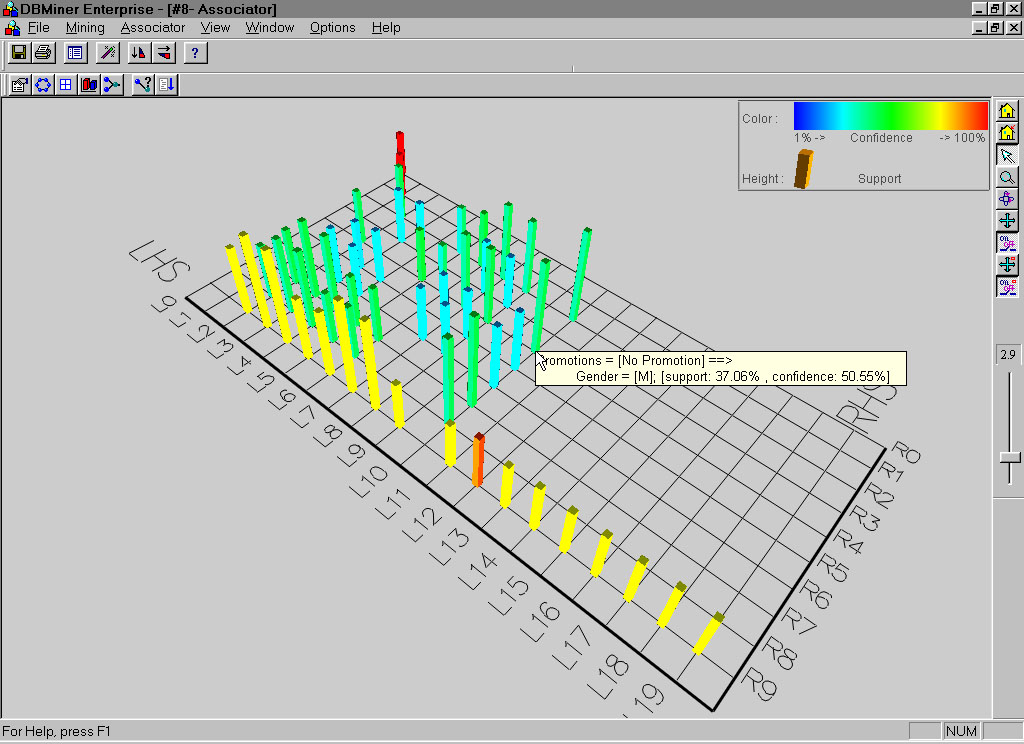
\includegraphics[width=0.6\textwidth]{img/assoc_rules1.jpg}
	}
\end{frame}

\begin{frame}{Visualization of Association Rules: Plane Graph}
	\centering
	\scalebox{0.9}{
		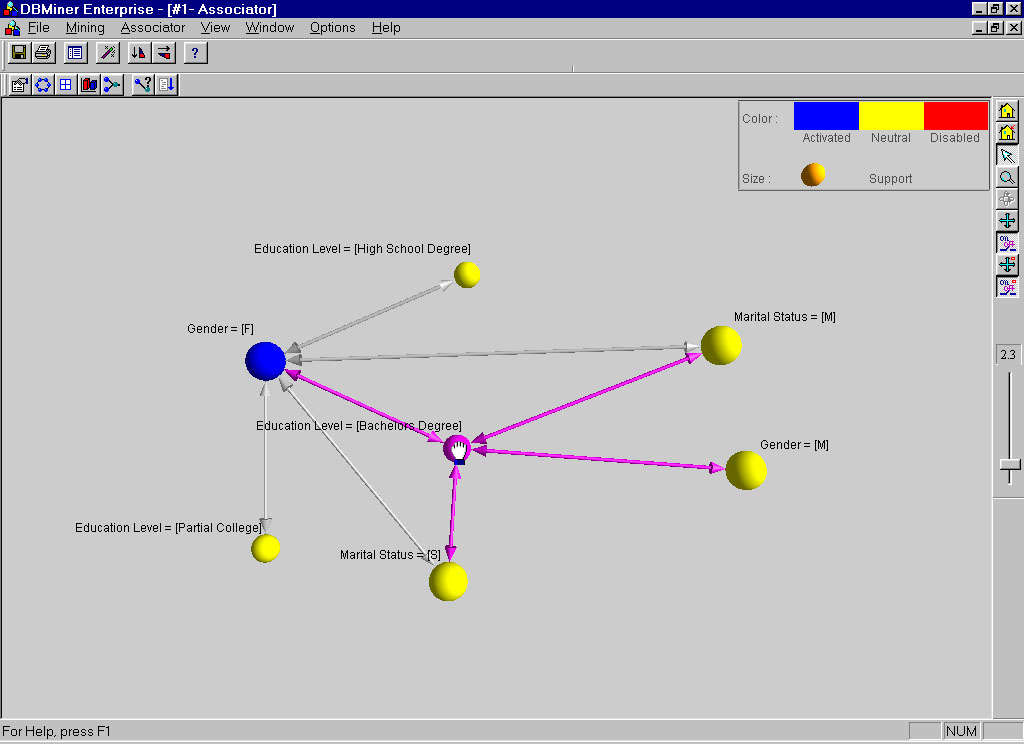
\includegraphics[width=0.6\textwidth]{img/assoc_rules2.jpg}
	}
\end{frame}

\begin{frame}{Visualization of Association Rules: SGI/MineSet 3.0}
	\centering
	\scalebox{0.9}{
		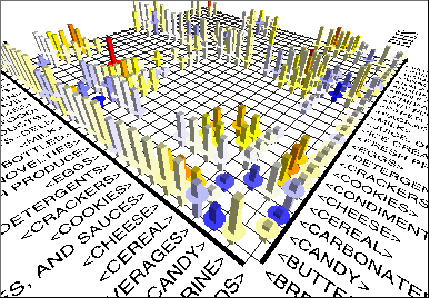
\includegraphics[width=0.6\textwidth]{img/assoc_rules3.png}
	}
\end{frame}
